\section{Experimental Evaluation}
\label{sec:experimental-evaluation}

We evaluate whether command and action features retrieve same-task trajectories across execution modes, and whether an execution-mode score adds value beyond behavioral similarity. These experiments make execution-aware correlation measurable under fixed, held-out candidate sets.

\subsection{Motivation: execution mode as activity context}
\label{sec:motivation}

Threat analysis distinguishes grouping observed behavior into a campaign from attributing that campaign to an organization. STIX 2.1 defines a Campaign as malicious activities or attacks grouped over time and targets; an Intrusion Set groups related behaviors and resources believed to be orchestrated by one organization, and attribution is represented as an explicit relationship. This separation makes activity association a meaningful analysis target in its own right. Systems such as \href{https://www.seclab.cs.sunysb.edu/seclab/pubs/holmes19.pdf}{HOLMES} correlate audit behavior and information-flow relationships into multi-stage campaign evidence, while \href{https://arxiv.org/abs/2312.09321}{OSTINATO} compares provenance-graph behavior across hosts to extend attack-activity candidates. MITRE ATT\&CK likewise describes procedures as the specific implementations through which adversaries perform techniques, including operational behavior and tools.

Execution mode is now visible in campaign accounts. The 2025 report on the activity catalogued by MITRE as Campaign C0062 describes human operators coordinating Claude Code agents through MCP tools across reconnaissance, exploitation, lateral movement, and collection. The report places human direction and Agent-mediated operations within one campaign, making the mode of execution part of the behavior evidence available to investigators.

We bring execution mode into behavior-based activity association as an explicit evidence dimension. The study asks whether log-derived mode estimates help analysts interpret operational differences, recover cross-mode links, and keep unrelated activity apart. This positions participation at the activity-analysis layer and creates a reproducible path toward richer AI-era threat profiles; the evaluation protocol specifies the scope of the available public traces.

\subsection{Data and protocol}
\label{sec:data-protocol}

The traces come from the public Cyber Task Horizons release (pinned commit \texttt{178c0da1800f9c07311e1b8d6c61dd8104e7b4ae}; \href{https://github.com/lyptus-research/cyber-task-horizons-data/tree/178c0da1800f9c07311e1b8d6c61dd8104e7b4ae}{data and evaluation logs}; \href{https://lyptusresearch.org/research/offensive-cyber-time-horizons}{collection methodology}). The release combines model evaluations across seven offensive-cyber benchmarks with an expert study covering 291 tasks and ten professionals. We select the three CTF suites for which the release provides both human and Agent records for overlapping task IDs. InterCode-CTF adapts 100 PicoCTF objectives into interactive tasks represented by an instruction, assets, and a hidden flag (\href{https://papers.nips.cc/paper_files/paper/2023/file/4b175d846fb008d540d233c188379ff9-Paper-Datasets_and_Benchmarks.pdf}{InterCode paper}); CyBench contains 40 professional-level challenges from four competitions (\href{https://arxiv.org/abs/2408.08926}{CyBench paper}); NYU CTF Bench compiles diverse challenges from established competitions (\href{https://proceedings.neurips.cc/paper_files/paper/2024/hash/69d97a6493fbf016fff0a751f253ad18-Abstract-Datasets_and_Benchmarks_Track.html}{NeurIPS 2024 paper}).

The evaluated intersection contains 177 parseable, non-empty traces from 40 benchmark--task groups: 57 expert terminal traces and 120 Agent traces. Table~\ref{tab:dataset-counts} gives the per-suite counts. Each task ID denotes a CTF challenge, so it provides a reproducible same-task label for retrieval; it does not identify a shared intrusion, operator, or campaign. The collection runs human experts and model agents in the same task containers, but records them through different interfaces: human `.input` terminal transcripts and structured Agent tool calls. The released human study instructed experts not to use AI, while noting that remote collection cannot strictly verify compliance. We therefore use the release's human/Agent labels as trace-source labels, not as independently verified decision-author identity.

For both record types, we extract allowlisted command names and map them to coarse action categories. We exclude prompts, task descriptions, outputs, answers, model names, timestamps, and paths from association features. The selected Agent traces contain 300 Python tool calls; these are omitted from the primary command representation. Exact file hashes, selected task IDs, latest-run deduplication rules, and aggregate counts are recorded in the repository manifests and \texttt{results/crossbenchmark\_exploration.json}; raw traces remain local under the upstream data terms.

All records for a \texttt{benchmark/task\_id} remain in one of five outer folds. The primary historical-gallery protocol holds query tasks out of model fitting but ranks against all same-benchmark tasks; thus, training-fold traces can appear as negative gallery candidates. Vocabulary, TF--IDF weights, ProcGrep patterns, mode classifiers, and association rankers are fit on training tasks only. Training-gallery mode scores are inner-fold out-of-fold predictions; held-out query scores come from the outer-fold model. A stricter gallery protocol restricts both queries and candidate tasks to the outer held-out fold. We report benchmark-macro Recall@1, mean reciprocal rank (MRR), and query AUC. Confidence intervals use 5,000 task-cluster bootstrap replicates, stratified by benchmark; each benchmark contributes equally to the macro-average. Paired contrasts use the same eligible query tasks within each gallery protocol.

\subsection{Behavioral traces retrieve same-task Agent activity above random ranking}
\label{sec:cross-mode-retrieval}

The strongest simple representation is the ordered coarse-action bigram model, with Human-to-Agent Recall@1 of 0.414 (95\% task-cluster CI [0.245, 0.576]), MRR 0.561, and query AUC 0.733. It reaches the highest point estimate among the four representation baselines and matches the mode-aware prototype's Recall@1 point estimate. The other simple baselines obtain Recall@1 values of 0.347 for command unigrams, 0.265 for ordered command bigrams, and 0.287 for ProcGrep local patterns; their intervals and full metrics appear in Appendix~\ref{app:complete-results}. The benchmark-macro random-ranking baseline is 0.116.

The same ordering signal appears within each benchmark: ordered-action-bigram Recall@1 is 0.417 on CyBench (6 tasks; random 0.167), 0.111 on InterCode-CTF (27 tasks; random 0.037), and 0.714 on NYUCTF (7 tasks; random 0.143). The absolute values vary substantially across suites, so the pooled result indicates task-discriminative structure under these same-benchmark negatives, with benchmark-specific difficulty shaping performance. Figure~\ref{fig:retrieval} reports the task-cluster intervals and complete representation comparison.

\begin{figure}[tb]
  \centering
  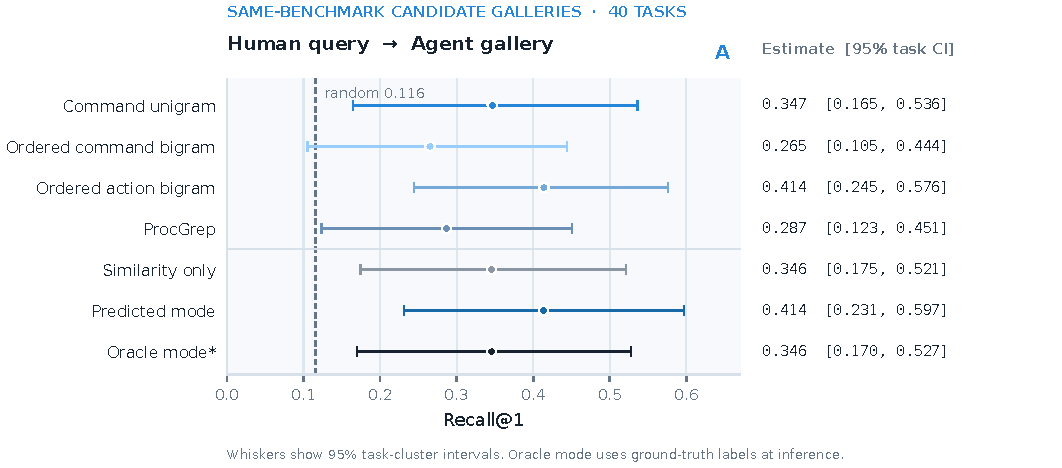
\includegraphics[width=\linewidth]{figure1_retrieval.pdf}
  \caption{Human-to-Agent same-task retrieval with same-benchmark hard negatives. Points show benchmark-macro Recall@1 and whiskers show 95\% task-cluster bootstrap intervals. The dashed line marks the macro random-ranking baseline (0.116). The oracle-mode row uses ground-truth mode labels at inference and is included only as a diagnostic. Task identity is a CTF challenge proxy, not an attack-activity label.}
  \label{fig:retrieval}
\end{figure}

\subsection{Execution-mode information has direction-dependent effects}
\label{sec:mode-effects}

Adding out-of-fold mode scores changes Human-to-Agent Recall@1 from 0.346 to 0.414 in the historical-gallery protocol, a paired gain of 0.068 across 40 task groups (95\% CI [\(-0.012\), 0.191]). Paired changes in MRR (0.039, CI [\(-0.006\), 0.100]) and query AUC (0.015, CI [\(-0.005\), 0.040]) also span zero. This point estimate is not specific to mode supervision: a fixed 11-feature command-length control reaches Recall@1 0.431, and the mode ranker trails it by 0.018 (paired 95\% CI [\(-0.071\), 0.025]). The oracle diagnostic uses true mode labels and returns Recall@1 0.346, equal to the similarity-only point estimate; because all Human-to-Agent pairs already have the same binary mode relation, this is not a general upper bound on mode-aware association.

The direction-specific result remains a caution: Human-to-Human Recall@1 decreases by 0.098 (95\% CI [\(-0.189\), \(-0.007\)]; 17 eligible task groups), while Agent-to-Agent cross-model and Agent-to-Human changes are small and uncertain. In the strict held-out-gallery protocol, mode-aware Human-to-Agent Recall@1 is 0.632 versus 0.638 for similarity alone (36 eligible query tasks; paired change \(-0.006\), 95\% CI [\(-0.019\), 0.000]). The random-ranking baseline also rises from 0.116 to 0.278 because the held-out gallery averages only 4.1 candidate tasks, so scores across gallery protocols are not directly comparable. Figure~\ref{fig:mode-effects} summarizes directional effects; Figure~\ref{fig:specificity-controls} shows the fixed controls and candidate-gallery sensitivity.

\begin{figure}[tb]
  \centering
  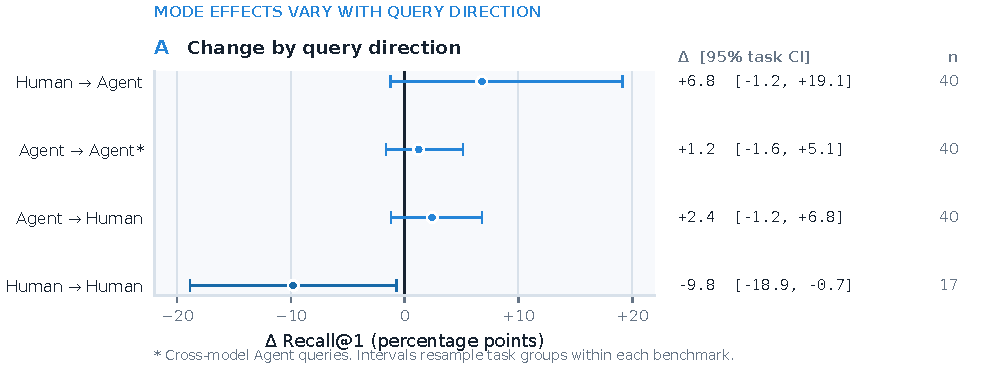
\includegraphics[width=\linewidth]{figure2_mode_effects.pdf}
  \caption{Paired change in Recall@1 after adding predicted execution-mode features to the similarity-only ranker. Positive values favor the mode-aware ranker. Intervals resample task groups within benchmark; \(n\) counts eligible independent task groups. Agent-to-Agent queries use different source models.}
  \label{fig:mode-effects}
\end{figure}

\subsection{Mode-label prediction measures trace separability, not actor identity}
\label{sec:mode-classification}

The command n-gram mode head obtains pooled-record balanced accuracy 0.863 (95\% CI [0.804, 0.915]), macro-F1 0.854, and ROC AUC 0.945 (95\% CI [0.917, 0.972]) on the 177 held-out traces. A command-count/action-mixture control reaches AUC 0.728, while benchmark identity alone reaches AUC 0.501. This pattern shows that the release's trace-source labels are predictable beyond benchmark identity. It also shows why the classifier cannot yet be interpreted as an actor detector: expert activity is recorded as terminal input and Agent activity as tool calls, so label and capture pathway are aligned. The result motivates a same-sensor evaluation in which operator and execution mode vary independently.

We next held each Agent model source out of every training fold and evaluated it only on task-held-out Human--Agent pairs. The command n-gram classifier retained a benchmark-macro balanced accuracy of 0.862 across the three withheld sources (95\% task-cluster CI [0.805, 0.912]); source-specific estimates were 0.820 for Claude Opus 4.6, 0.918 for Claude Sonnet 4.6, and 0.847 for GPT-5.5. Action-category n-grams reached 0.734 (95\% CI [0.666, 0.803]), and command-count/action-mix features reached 0.617 (95\% CI [0.558, 0.683]). The paired change against training with all sources was +0.018 (95\% CI [−0.034, +0.072]). These estimates describe transfer among three model sources within one release. In all 177 records, however, human labels come from terminal-input files and Agent labels from structured tool-call files, so this transfer test does not separate behavior from instrumentation. Full source-specific estimates and the provenance audit appear in Appendix~\ref{app:unseen-model}.

On a separate task-macro comparison, command-name TF--IDF with logistic regression obtains balanced accuracy 0.844 (95\% task-cluster CI [0.766, 0.915]), macro-F1 0.804, and ROC-AUC 0.957 [0.914, 0.992]. Coarse-action TF--IDF and fixed count/action features score lower in balanced accuracy (0.777 and 0.622); ExtraTrees improves the count/action baseline to 0.723. ExtraTrees has the lowest 10-bin ECE point estimate (0.073), while command TF--IDF has the lower Brier score (0.125). These are raw classifier scores without a fitted calibration stage. Figure~\ref{fig:local-model-comparison} presents the full grouped comparison. This task-macro protocol differs from the pooled-record estimate above (0.863) and should not be read as a direct paired comparison.

\begin{figure}[tb]
  \centering
  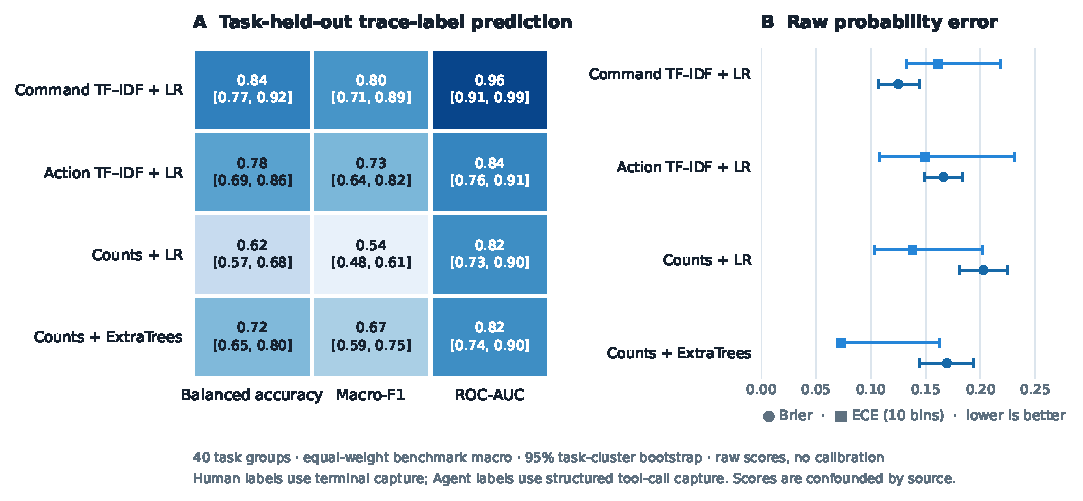
\includegraphics[width=\linewidth]{figureA7_local_model_comparison.pdf}
  \caption{Local trace-label baselines under task-grouped evaluation. The heatmap shows balanced accuracy, macro-F1, and ROC-AUC with 95\% task-cluster intervals. The right panel reports Brier and 10-bin ECE on raw, uncalibrated probabilities. Metrics macro-average tasks within each benchmark and weight benchmarks equally. Human terminal capture and Agent tool-call capture remain aligned with the target labels.}
  \label{fig:local-model-comparison}
\end{figure}

We also ran a post-hoc conditional label-permutation diagnostic with 999 refits. Labels were shuffled only among training traces within each task, preserving task composition, held-out labels, candidate sets, and pair truth. In the historical gallery, the observed mode-minus-similarity change was +0.068 Recall@1, and 5/999 shuffled outcomes met or exceeded it. In the held-out-only gallery, the observed change was −0.006, with 323/999 shuffled outcomes at least as large. The historical-gallery contrast is unusual relative to this conditional reference distribution, but this is not a causal test: within-task label exchangeability is unverified, the analysis is post hoc, and execution label is perfectly confounded with capture pathway. The strict-gallery result provides no corresponding positive signal. Figure~\ref{fig:mode-label-permutation} and Appendix~\ref{app:permutation} document the diagnostic.

\subsection{Resulting research claim}
\label{sec:resulting-claim}

Across the evaluated public traces, command features separate the release's Human and Agent record labels even when an Agent model family is withheld, but the resulting mode score does not show a stable improvement in cross-mode task retrieval: it does not outperform the length control in the historical gallery, and its point estimate is slightly lower than the similarity baseline in the held-out gallery. The main empirical finding is this separation between recognition and downstream utility. It turns execution mode into a measurable candidate context for activity profiles and shows why its value must be judged by association errors, not classification accuracy alone. Measuring the effect on actual activity links requires repeated executions under shared telemetry with independent activity identifiers.
